\begin{figure}
    \begin{center}
        % 
\includegraphics[width=0.5\textwidth]{papers/particles/figures/wavesim/particle_initial_state.png}
        \subfigure[]{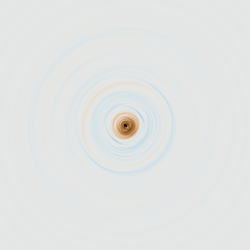
\includegraphics[width=0.45\textwidth]{./papers/particles/figures/simulations/particle_frames/frame_17.png}}\hfill%
% Alternativ könnte man zusätzlich noch diese Grafik einfügen:
        \subfigure[]{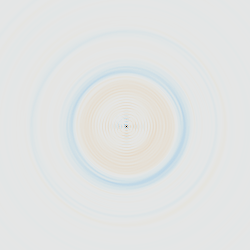
\includegraphics[width=0.45\textwidth]{./papers/particles/figures/simulations/particle_frames/frame_18.png}}
        \caption{Schlussendlicher Zerfall der Energieansammlung.}\label{particles:fig:partikel:abnehmen:zerfall}
    \end{center}
\end{figure}